% Use a modified ACM conference proceedings template
\documentclass[sigconf]{acmart}

% Disable some elements from ACM template
\setcopyright{none}
\settopmatter{printacmref=false,printfolios=false}
\renewcommand\footnotetextcopyrightpermission[1]{}

\acmConference[Machine Perception]{Machine Perception - ETH}{June 16}{2019}
% \acmConference[WOODSTOCK'18]{ACM Woodstock conference}{July 29-August 3, 2018}{City, State, Country}

\usepackage{booktabs} % For formal tables

\begin{document}
\title{Machine Perception Project 1: \\ Dynamic Gesture Recognition}

\author{Nicolas K{\"u}chler}\affiliation{}
\email{kunicola@student.ethz.ch}

\author{Yoel Zweig}\affiliation{}
\email{zweigy@student.ethz.ch}

\begin{abstract}

Deep neural networks have shown impressive results in the area of image classification, sometimes even outperforming humans.
At the moment, the performance in video classification is not on the same level. This is due to the additional temporal dimension which makes the problem much harder.
In this work, we tackle the task of classifying short video clips of 20 different Italian sign gestures using a combination of Convolutional Neural Networks (CNNs) and Recurrent Neural Networks (RNNs). The predictions of three networks with identical base architectures but slightly different configurations are combined in a majority voting ensemble to further improve accuracy.
Moreover, a variety of data augmentation and regularization techniques are used to prevent overfitting. 


\end{abstract}

\maketitle

\section{Introduction}

The goal of this project is to create a model capable of distinguishing 20 Italian sign gestures. The network is trained on a customized version of the ChaLearn dataset\cite{ChaLearn17}, which provides RGB, depth, segmentation mask and skeletal information. The dataset contains 9961 video clips, with 5722 in the training set, 1765 in the validation set and 2174 in the test set. Each clip has a length of 50-150 frames with a resolution of 80x80 pixels.

Since the dataset is relatively small for a task of this complexity, there is a danger of overfitting the network to the training data. To counteract this problem, we make heavy use of data augmentation and regularization techniques.

The high-level idea of our approach is to use a CNN to project each video frame to a low dimensional feature space and then use a bidirectional RNN with LSTM cells\cite{LSTM97} to capture temporal dependencies of the gestures. Finally, three such models are combined in an ensemble to improve classification accuracy. 


\section{Data Pre-Processing and Augmentation}\label{sec:data}

The RGB input video is normalized to zero-mean and unit variance. Since the background does not contain any relevant information, we apply the segmentation mask to every RGB frame of the video. This results in a black background for all RGB frames.
Instead of using the whole clip, we extract a random 64-frame subsequence every epoch. This is inspired by \cite{Pigou16} because a gesture is generally only about 20-50 frames long. Additionally, this generates more diverse training data.

At the start of every epoch, the data augmentation techniques listed below are applied to the training set using parameters chosen uniformly at random from an interval. As a result, the network always receives slightly different samples which helps generalization. 

We apply temporal augmentation by sampling a factor in the interval [0.8, 1.2] and slow down respectively speedup the video by this factor.
Additionally, we perform color augmentation by randomly perturbing the RGB channels through adjusting brightness [-0.2, 0.2], changing saturation [0.6, 1.6] and modifying contrast [0.7, 1] using the functions from tf.image.
Moreover, each sample is flipped horizontally with a probability of 0.5.
Finally, every video is randomly cropped and rescaled such that at least of 90\% of both height and width remain in the video. This results in both a translation and a zoom.


\section{Model}\label{sec:model}

After online pre-processing and data augmentation, the videos are fed into a CNN to extract spatial features from each frame. Afterwards, the spatial features are fed into a RNN to extract temporal information. Finally, a dense layer with a softmax activation function is used to calculate the class probabilities from the output of the RNN. 
Figure \ref{fig:architecture} gives an overview over the complete architecture.

\begin{figure*}
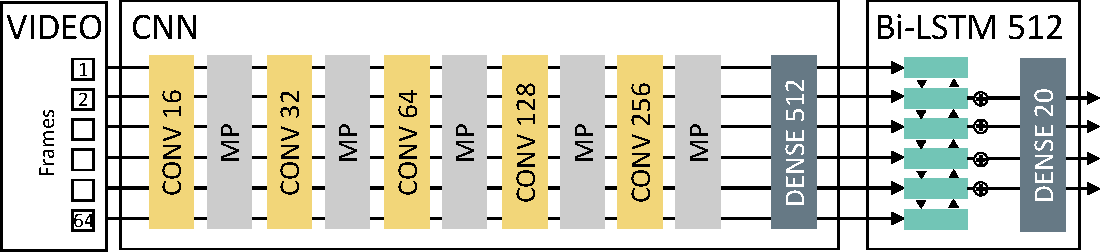
\includegraphics[width=0.9\textwidth]{architecture.pdf}
\caption{Model Architecture: Frames of a video are fed separately through a CNN to extract spatial features. Afterwards, the bidirectional LSTM is used to infer temporal dependencies. Only the middle 32 frames are used for prediction.}\label{fig:architecture}
\end{figure*}


\subsection{CNN}

The CNN architecture consists of five blocks, each composed of a convolutional layer with a leaky ReLU (alpha=0.3) activation function followed by a max pooling layer. All blocks use 3x3 convolution kernels and 2x2 max pooling with a stride of 2. Starting with 16 filters, the amount of filters doubles in every successive block.
A single dense layer of size 512 concludes the CNN model. In the dense layer, we use dropout in the range of [0.4, 0.5] to reduce overfitting.

The overall architecture can be summarized in the following way: C(16)-P-C(32)-P-C(64)-P-C(128)-P-C(256)-P-D(512)


\subsection{RNN}

We use a bidirectional LSTM architecture with 512 units to extract temporal information from the CNN output.  The forward and backward directions of the RNN are combined by adding the output for each timestep together.

A dense layer with dropout in the range of [0.4, 0.5] projects the RNN output of every time step to the 20 classes.  The same architecture was successfully used in \cite{Pigou16}.


\section{Training}

The loss is calculated by using the same sequence label for each time-step of a video clip but excluding a warm-up of 16 frames in both directions. The exclusion of the warm-up is motivated by the fact that a few frames are insufficient to recognize the gestures and therefore it is better to ignore the RNN output of the first frames in both directions \cite{Pigou16}. 

In order to combat the exploding gradient problem, we clip gradients with a norm larger than a certain value.

The cross-entropy loss is minimized using the Adam optimizer with a learning rate of 0.0005 and a batch size of 16. The learning rate has an exponential decay rate of 0.97 every 500 steps. We trained for a minimum of 28 epochs and implemented early stopping based on validation accuracy.
The models were trained on the ETH Leonhard cluster using a single GeForce GTX 1080 graphics card for approximately 4 hours.

As described in section \ref{sec:data}, we only train the network on sub-clips with 64 frames.
In evaluation mode, we ensure that the whole video length is considered for the prediction using a sliding window approach. For every test sample, 16 evenly spaced subsequences of 64 frames are extracted and fed separately to the model. The 16 separate predictions are combined using an ensemble approach by adding all logits. 


\section{Results}

The final and best submission is a majority vote ensemble of the three best individual submissions. In case of a tie, the prediction of the model with the best individual performance (part 2) is used as a tie-breaker. 

\begin{table}[h!]
  \caption{Experiment Configuration: Differences}
  \label{tab:exp-diff}
  \begin{tabular}{lccc}
    \toprule
    Configuration & Part 1 & Part 2 & Part 3 \\
    \midrule
    Gradient Clipping Norm & 1 & 10 & 10 \\
    Training on Validation Set & true & false & false \\
    CNN Dropout & 0.5 & 0.5 & 0.4 \\
    LSTM Dropout & 0.4 & 0.5 & 0.4 \\
    LSTM Layers & 1 & 2 & 1 \\
  \bottomrule
\end{tabular}
\end{table}

The model architecture and hyperparameters of the three different parts of the ensemble are as described in section \ref{sec:model} but with a few configuration differences highlighted in table \ref{tab:exp-diff}.

\begin{table}[h!]
  \caption{Experimental Results}
  \label{tab:exp-res}
  \begin{tabular}{lcc}
    \toprule
    Experiment & Valid Accuracy & Test Accuracy \\
    \midrule
    Sample Baseline & - & 0.4765 \\
    Easy Baseline &  - & 0.7553 \\
    Hard Baseline & - & 0.8326 \\
    \midrule
    Part 1: Train on Valid & - & 0.8132    \\
    Part 2: Stack LSTM  & 0.6992 & 0.8399           \\
    Part 3: Less Dropout & 0.6980 & 0.8142          \\
    \textbf{Vote Ensemble}  & - & \textbf{0.8546}  \\
  \bottomrule
\end{tabular}
\end{table}


Table \ref{tab:exp-res} summarizes the experimental results of the final submission and compares them to the provided baselines.

All individual models are better than the easy baseline but only the model with two LSTM layers manages to marginally beat the hard baseline on the public test set.
Combining the three models in an ensemble approach boosts the performance well above the hard baseline.
We only performed a small ensemble of three similar models. However, our results suggest that already with these small configuration changes and the randomness in the training process there is enough variety such that the classifier can benefit from the ensemble approach.

Another observation which was consistent across all experiments is that the validation set poses a much harder challenge than the public part of the test set. The accuracy scores are on average a bit more than 10\% lower on the validation set.

It should be noted that the final submission has been trained using only RGB data and the segmentation mask. We experimented with different approaches to make use of depth and skeleton data but failed to improve accuracy. More information on the other experiments can be found in appendix \ref{appendix}.


\section{Conclusions}

We have successfully combined a CNN and a RNN for spatial- and temporal feature extraction. Using this approach, we have built a classifier for Italian sign gestures from videos and demonstrated its effectiveness on the customized ChaLearn dataset\cite{ChaLearn17}.

The problem of overfitting due to the small size of the training set compared to the large dimensionality of the data remains. Nevertheless, we confirm the results of \cite{Pigou16} that data augmentation is integral in combating this.

We have shown the usefulness of building an ensemble of multiple models to boost performance significantly.
This suggests that in future work it might be beneficial to build an ensemble with more than three classifiers.
Further exploration is needed on what kind of model differences are helpful in such an ensemble.
A wide range of possibilities exists such as training on different training-validation splits, using different architectures or using different input data.

Even though the approaches described in appendix \ref{appendix} did not yield improved performances in our experiments individually, some of them could be further tuned and prove beneficial in an ensemble.


\appendix
%Appendix A

\section{Further Experiments}\label{appendix}

During the work on the project, we explored a few directions which did not lead to better results, but we list them here for completeness.

\subsection{Larger CNN}
The use of a larger CNN similar to the one used in \cite{Pigou16}, \cite{Simonyan15} did not result in a better performance.
The network architecture we evaluated can be described in the following way: C(16)-C(16)-P-C(32)-C(32)-P-C(64)-C(64)-P-C(128)-C(128)-P-C(256)-C(256)-P-D(512).

\subsection{Temporal and Spatial Convolutions}
We could not reproduce the results from \cite{Pigou16} with the spatial- and temporal (2+1)D-convolution architecture due to convergence problems.

The model converged using a smaller version of the architecture with only one instead of two (2+1)D-convolutional layers per block.
However, the temporal convolutions did not appear to benefit the model in our experiments compared to the CNN architecture described in section \ref{sec:model}.

\subsection{Depth}
Using RGB-Depth input as in \cite{Pigou16} resulted in covergence issues.
These issues were resolved by introducing batch normalization after every convolutional layer. However, the overall performance did not benefit from the additional channel.

\subsection{Hands CNN}
Studying the confusion matrix during the training process has shown that the model struggles sometimes to discriminate between gestures with similar arm movement but different hand shapes. 

To support the network we use the skeleton information to extract two 16x16 patches centered around the two hands and feed them to a small CNN. The resulting hand features are concatenated with the features from the RGB image and fed to the bidirectional LSTM.

Even though training the model only on the hands showed promising results, the anticipated increase in accuracy did not occur when fusing the features of the hand model with the RGB features.

\subsection{Additional Augmentation}
Inspired by \cite{Pigou16} we implemented random translation, rotation and shearing as additional data augmentations. These additional augmentations did not boost performance but slowed down the training process, since they are computationally expensive.

\subsection{Concat Bidirectional Output}
Instead of adding the outputs from the forward and backward LSTM frame wise, we tried to concatenate them.
In theory, this should make the model more powerful. However, in our experiments, this setup did not converge.

\subsection{Joint Trajectory Maps}
Joint Trajectory Maps is a method to encode spatio-temporal information carried in sequences of skeleton data into 2D-images \cite{JointTrajectoryMaps16}.
Spatial information of the joint is captured by the dot position in the image and the temporal information is captured by the dot color.

We create a separate joint trajectory map for hand, elbow, shoulder, spine and head of every video clip.
The resulting maps are concatenated and fed into a standard CNN for classification.

\begin{figure}[h!]
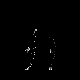
\includegraphics{joint-hands.png}
\caption{Example of a joint trajectory map of two hands}
\end{figure}

A problem of the approach is that the shape of some body parts cannot be fully represented by the given skeletal data (e.g. hand shape).
Still, the general approach seems to hold potential in particular when considering that the problem of video classification can be reduced to a problem of image classification.

\begin{acks}
The authors would like to thank Emre Aksan for the well-structured template code and the Machine Perception team for organizing the project.
\end{acks}

\bibliographystyle{ACM-Reference-Format}
\bibliography{bibliography}

\end{document}
